\documentclass[12pt,a4paper]{scrartcl}
\usepackage{ifpdf}
\usepackage[utf8]{inputenc}
\usepackage[ngerman]{babel}
\usepackage{amsmath}
\usepackage{amssymb}
\usepackage{fancyhdr}
\usepackage{listings}
\usepackage{color}
\usepackage{pdfpages}
\usepackage{stmaryrd}

\pagestyle{fancy}
\fancyhead{}
\fancyfoot{}
\fancyhead[LO,LE]{Johannes Hedtrich, Christopher Hlubek}
\fancyhead[RO,RE]{Serie 04}
\fancyfoot[CO,CE]{\thepage}

\title{Serie 04}
\author{Johannes Hedtrich, Christopher Hlubek}
\date{\today}
\begin{document}

\section*{4.3}
Modellierung des Dominoproblems mit Hilfe der Erfüllbarkeit einer aussagenlogischer Formelmenge
mit Variablen der Form $X_{ij}^f$:

\paragraph{Die Stelle $(i, j)$ der Parkettierung ist besetzt:}
\[
\varphi_{ij}^S = \bigwedge_{f,g\in S: f \neq g} \left( X_{ij}^f \leftrightarrow \neg X_{ij}^g \right)
\]

\paragraph{Alle Teile um $(i, j)$ passen:}
\begin{align*}
\psi_{ij}^S &= \bigvee_{f\in S} \Big( X_{ij}^f\\
&\wedge \bigvee_{g\in S:f(0) = g(2)} X_{(i+1)j}^g\\
&\wedge \bigvee_{g\in S:f(1) = g(3)} X_{i(j+1)}^g\\
&\wedge \bigvee_{g\in S:f(2) = g(0) \dot \wedge i>0} X_{(i-1)j}^g\\
&\wedge \bigvee_{g\in S:f(3) = g(1), j>0} X_{i(j-1)}^g \Big)
\end{align*}

\paragraph{Parkettierung korrekt:}
\[
\Phi^S = \bigwedge_{0<i,0<j}\lbrace \varphi_{ij}^S \wedge \psi_{ij}^S \rbrace
\]

\section*{4.4}
\subsection*{Voraussetzung:}

Seien $\varphi, \psi, \theta \in F_{AL}$.

\subsection*{Behauptung:}
Die Formeln
\begin{enumerate}
  \item[(a)] $\varphi_a = \neg((((\theta \wedge \varphi) \wedge \neg \varphi) \vee \psi) \rightarrow \psi)$
  \item[(b)] $\varphi_b = ((\neg (\neg \psi \rightarrow \neg \varphi) \wedge (\varphi \rightarrow \psi)) \wedge \neg(\varphi \wedge \neg \psi))$
  \item[(c)] $\varphi_c = (((\psi \wedge \varphi) \vee \theta) \wedge ((\neg \varphi \wedge \neg \theta) \vee \neg(\neg \psi \rightarrow \theta)))$
\end{enumerate}
sind unerfüllbar.

\subsection*{Beweis}

Idee: Zeige $\varphi \equiv 0$\\
O.B.d.A. gelte im Folgenden $X_0 \not\in \textrm{vars}(\varphi) \cup \textrm{vars}(\psi) \cup \textrm{vars}(\theta)$.

\setcounter{equation}{-1}
\begin{align}
  \varphi_a
    & =\neg ((((\theta \wedge \varphi) \wedge \neg \varphi) \vee \psi) \rightarrow \psi) \\
    & \equiv \neg(((\theta \wedge (\varphi \wedge \neg \varphi)) \vee \psi) \rightarrow \psi) \\
    & \equiv \neg(((\theta \wedge 0) \vee \psi) \rightarrow \psi) \\
    & \equiv \neg((0 \vee \psi) \rightarrow \psi) \\
    & \equiv \neg(\psi \rightarrow \psi) \\
    & \equiv \neg(\neg \psi \vee \psi) \\
    & \equiv \neg \neg \psi \wedge \neg \psi \\
    & \equiv \psi \wedge \neg \psi \\
    & \equiv 0
\end{align}

\begin{enumerate} 
\item 2. Ersetzungslemma:
    $i = 0$, $\varphi_s = \neg ((X_0 \vee \psi) \rightarrow \psi)$, $\psi_s = ((\theta \wedge \varphi) \wedge \neg \varphi)$, $\psi'_s = (\theta \wedge (\varphi \wedge \neg \varphi))$.
    $\psi_s \equiv \psi'_s$ gilt nach Assoziativität.
  \item 2. Ersetzungslemma:
    $i = 0$, $\varphi_s = \neg(((\theta \wedge X_0) \vee \psi) \rightarrow \psi)$, $\psi_s = (\varphi \wedge \neg \varphi)$, $\psi'_s = 0$.
    $\psi_s \equiv \psi'_s$ gilt nach Tertium non datur.
  \item 2. Ersetzungslemma:
    $i = 0$, $\varphi_s = \neg((X_0 \vee \psi) \rightarrow \psi)$, $\psi_s = (\theta \wedge 0)$, $\psi'_s = 0$.
    $\psi_s \equiv \psi'_s$ gilt nach Größtes und kleinstes Element.
  \item 2. Ersetzungslemma:
    $i = 0$, $\varphi_s = \neg((0 \vee \psi) \rightarrow \psi)$, $\psi_s = (0 \vee \psi)$, $\psi'_s = \psi$.
    $\psi_s \equiv \psi'_s$ gilt nach Neutrales Element.
  \item 2. Ersetzungslemma:
    $i = 0$, $\varphi_s = \neg X_0$, $\psi_s = (\psi \rightarrow \psi)$, $\psi'_s = (\neg \psi \vee \psi)$.
    $\psi_s \equiv \psi'_s$ gilt nach Konditionalelimination.
  \item De Morgan
  \item 2. Ersetzungslemma:
    $i = 0$, $\varphi_s = X_0 \wedge \neg \psi$, $\psi_s = \neg \neg \psi$, $\psi'_s = \psi$.
    $\psi_s \equiv \psi'_s$ gilt nach Doppelte Negation.
  \item Tertium non datur
\end{enumerate}

\setcounter{equation}{-1}
\begin{align}
  \varphi_b 
    & = ((\neg (\neg \psi \rightarrow \neg \varphi) \wedge (\varphi \rightarrow \psi)) \wedge \neg(\varphi \wedge \neg \psi)) \\
    & \equiv ((\neg (\neg \neg \psi \vee \neg \varphi) \wedge (\varphi \rightarrow \psi)) \wedge \neg(\varphi \wedge \neg \psi)) \\
    & \equiv ((\neg (\neg \neg \psi \vee \neg \varphi) \wedge (\neg \varphi \vee \psi)) \wedge \neg(\varphi \wedge \neg \psi)) \\
    & \equiv ((\neg (\psi \vee \neg \varphi) \wedge (\neg \varphi \vee \psi)) \wedge \neg(\varphi \wedge \neg \psi)) \\
    & \equiv (((\neg \psi \wedge \neg \neg \varphi) \wedge (\neg \varphi \vee \psi)) \wedge \neg(\varphi \wedge \neg \psi)) \\
    & \equiv (((\neg \psi \wedge \varphi) \wedge (\neg \varphi \vee \psi)) \wedge \neg(\varphi \wedge \neg \psi)) \\
    & \equiv ((\neg \psi \wedge (\varphi \wedge (\neg \varphi \vee \psi))) \wedge \neg(\varphi \wedge \neg \psi)) \\
    & \equiv ((\neg \psi \wedge ((\varphi \wedge \neg \varphi) \vee (\varphi \wedge \psi))) \wedge \neg(\varphi \wedge \neg \psi)) \\
    & \equiv ((\neg \psi \wedge (0 \vee (\varphi \wedge \psi))) \wedge \neg(\varphi \wedge \neg \psi)) \\
    & \equiv ((\neg \psi \wedge (\varphi \wedge \psi)) \wedge \neg(\varphi \wedge \neg \psi)) \\
    & \equiv (((\neg \psi \wedge \psi) \wedge \varphi) \wedge \neg(\varphi \wedge \neg \psi)) \\
    & \equiv ((0 \wedge \varphi) \wedge \neg(\varphi \wedge \neg \psi)) \\
    & \equiv (0 \wedge \neg(\varphi \wedge \neg \psi)) \\
    & \equiv 0
\end{align}

\begin{enumerate} 
  \item Konditionalelimination \& 2. Ersetzungslemma
  \item Konditionalelimination \& 2. Ersetzungslemma
  \item Doppelte Negation \& 2. Ersetzungslemma
  \item De Morgan \& 2. Ersetzungslemma
  \item Doppelte Negation \& 2. Ersetzungslemma
  \item Assoziativität \& 2. Ersetzungslemma
  \item Distributivität \& 2. Ersetzungslemma
  \item Tertium non datur \& 2. Ersetzungslemma
  \item Neutrales Element \& 2. Ersetzungslemma
  \item Assoziativität \& 2. Ersetzungslemma
  \item Tertium non datur \& 2. Ersetzungslemma
  \item Größtes und kleinstes Element \& 2. Ersetzungslemma
  \item Größtes und kleinstes Element
\end{enumerate}

\setcounter{equation}{-1}
\begin{align}
  \varphi_c 
    & = (((\psi \wedge \varphi) \vee \theta) \wedge ((\neg \varphi \wedge \neg \theta) \vee \neg(\neg \psi \rightarrow \theta))) \\
    & \equiv (((\psi \wedge \varphi) \vee \theta) \wedge ((\neg \varphi \wedge \neg \theta) \vee \neg(\neg \neg \psi \vee \theta))) \\
    & \equiv (((\psi \wedge \varphi) \vee \theta) \wedge ((\neg \varphi \wedge \neg \theta) \vee \neg(\psi \vee \theta))) \\
    & \equiv (((\psi \wedge \varphi) \vee \theta) \wedge ((\neg \varphi \wedge \neg \theta) \vee (\neg \psi \wedge \neg \theta))) \\
    & \equiv (((\psi \wedge \varphi) \vee \theta) \wedge (((\neg \varphi \wedge \neg \theta) \vee \neg \psi) \wedge ((\neg \varphi \wedge \neg \theta) \vee \neg \theta))) \\
    & \equiv (((\psi \wedge \varphi) \vee \theta) \wedge (((\neg \varphi \wedge \neg \theta) \vee \neg \psi) \wedge \neg \theta)) \\
    & \equiv (((\psi \wedge \varphi) \vee \theta) \wedge (((\neg \varphi \vee \neg \psi) \wedge (\neg \theta \vee \neg \psi)) \wedge \neg \theta)) \\
    & \equiv (((\psi \wedge \varphi) \vee \theta) \wedge ((\neg \varphi \vee \neg \psi) \wedge ((\neg \theta \vee \neg \psi) \wedge \neg \theta))) \\
    & \equiv (((\psi \wedge \varphi) \vee \theta) \wedge ((\neg \varphi \vee \neg \psi) \wedge \neg \theta)) \\
    & \equiv (((\psi \vee \theta) \wedge (\varphi \vee \theta)) \wedge ((\neg \varphi \vee \neg \psi) \wedge \neg \theta)) \\
    & \equiv (((\psi \vee \theta) \wedge (\varphi \vee \theta)) \wedge ((\neg \varphi \wedge \neg \theta) \vee (\neg \psi \wedge \neg \theta))) \\
    & \equiv ((\psi \vee \theta) \wedge ((\varphi \vee \theta) \wedge ((\neg \varphi \wedge \neg \theta) \vee (\neg \psi \wedge \neg \theta)))) \\
    & \equiv ((\psi \vee \theta) \wedge (((\varphi \vee \theta) \wedge (\neg \varphi \wedge \neg \theta)) \vee ((\varphi \vee \theta) \wedge (\neg \psi \wedge \neg \theta)))) \\
    & \equiv ((\psi \vee \theta) \wedge ((((\varphi \vee \theta) \wedge \neg \varphi) \wedge \neg \theta) \vee ((\varphi \vee \theta) \wedge (\neg \psi \wedge \neg \theta)))) \\
    & \equiv ((\psi \vee \theta) \wedge ((((\varphi \wedge \neg \varphi) \vee (\theta \wedge \neg \varphi)) \wedge \neg \theta) \vee ((\varphi \vee \theta) \wedge (\neg \psi \wedge \neg \theta)))) \\
    & \equiv ((\psi \vee \theta) \wedge (((0 \vee (\theta \wedge \neg \varphi)) \wedge \neg \theta) \vee ((\varphi \vee \theta) \wedge (\neg \psi \wedge \neg \theta)))) \\
    & \equiv ((\psi \vee \theta) \wedge (((\theta \wedge \neg \varphi) \wedge \neg \theta) \vee ((\varphi \vee \theta) \wedge (\neg \psi \wedge \neg \theta)))) \\
    & \equiv ((\psi \vee \theta) \wedge (((\theta \wedge \neg \theta) \wedge \neg \varphi) \vee ((\varphi \vee \theta) \wedge (\neg \psi \wedge \neg \theta)))) \\
    & \equiv ((\psi \vee \theta) \wedge ((0 \wedge \neg \varphi) \vee ((\varphi \vee \theta) \wedge (\neg \psi \wedge \neg \theta)))) \\
    & \equiv ((\psi \vee \theta) \wedge (0 \vee ((\varphi \vee \theta) \wedge (\neg \psi \wedge \neg \theta)))) \\
    & \equiv ((\psi \vee \theta) \wedge ((\varphi \vee \theta) \wedge (\neg \psi \wedge \neg \theta))) \\
    & \equiv ((\psi \vee \theta) \wedge ((\varphi \wedge (\neg \psi \wedge \neg \theta)) \vee (\theta \wedge (\neg \psi \wedge \neg \theta)))) \\
    & \equiv ((\psi \vee \theta) \wedge (\varphi \wedge (\neg \psi \wedge \neg \theta))) \\
    & \equiv ((\psi \wedge (\varphi \wedge (\neg \psi \wedge \neg \theta))) \vee (\theta \wedge (\varphi \wedge (\neg \psi \wedge \neg \theta)))) \\
    & \equiv (0 \vee 0) \\
    & \equiv 0
\end{align}

\begin{enumerate} 
  \item Konditionalelimination \& 2. Ersetzungslemma
  \item Doppelte Negation \& 2. Ersetzungslemma
  \item De Morgan \& 2. Ersetzungslemma
  \item Distributivität \& 2. Ersetzungslemma
  \item Absorption \& 2. Ersetzungslemma
  \item Distributivität \& 2. Ersetzungslemma
  \item Assoziativität \& 2. Ersetzungslemma
  \item Absorption \& 2. Ersetzungslemma
  \item Distributivität \& 2. Ersetzungslemma
  \item Distributivität \& 2. Ersetzungslemma
  \item Assoziativität \& 2. Ersetzungslemma
  \item Distributivität \& 2. Ersetzungslemma
  \item Assoziativität \& 2. Ersetzungslemma
  \item Distributivität \& 2. Ersetzungslemma
  \item Tertium non datur \& 2. Ersetzungslemma
  \item Neutrales Element \& 2. Ersetzungslemma
  \item Assoziativität \& 2. Ersetzungslemma
  \item Tertium non datur \& 2. Ersetzungslemma
  \item Größtes und kleinstes Element \& 2. Ersetzungslemma
  \item Neutrales Element \& 2. Ersetzungslemma
  \item Distributivität \& 2. Ersetzungslemma
  \item analog wie 17 - 20
  \item Distributivität \& 2. Ersetzungslemma
  \item 2mal analog zu 17 - 20
\end{enumerate}

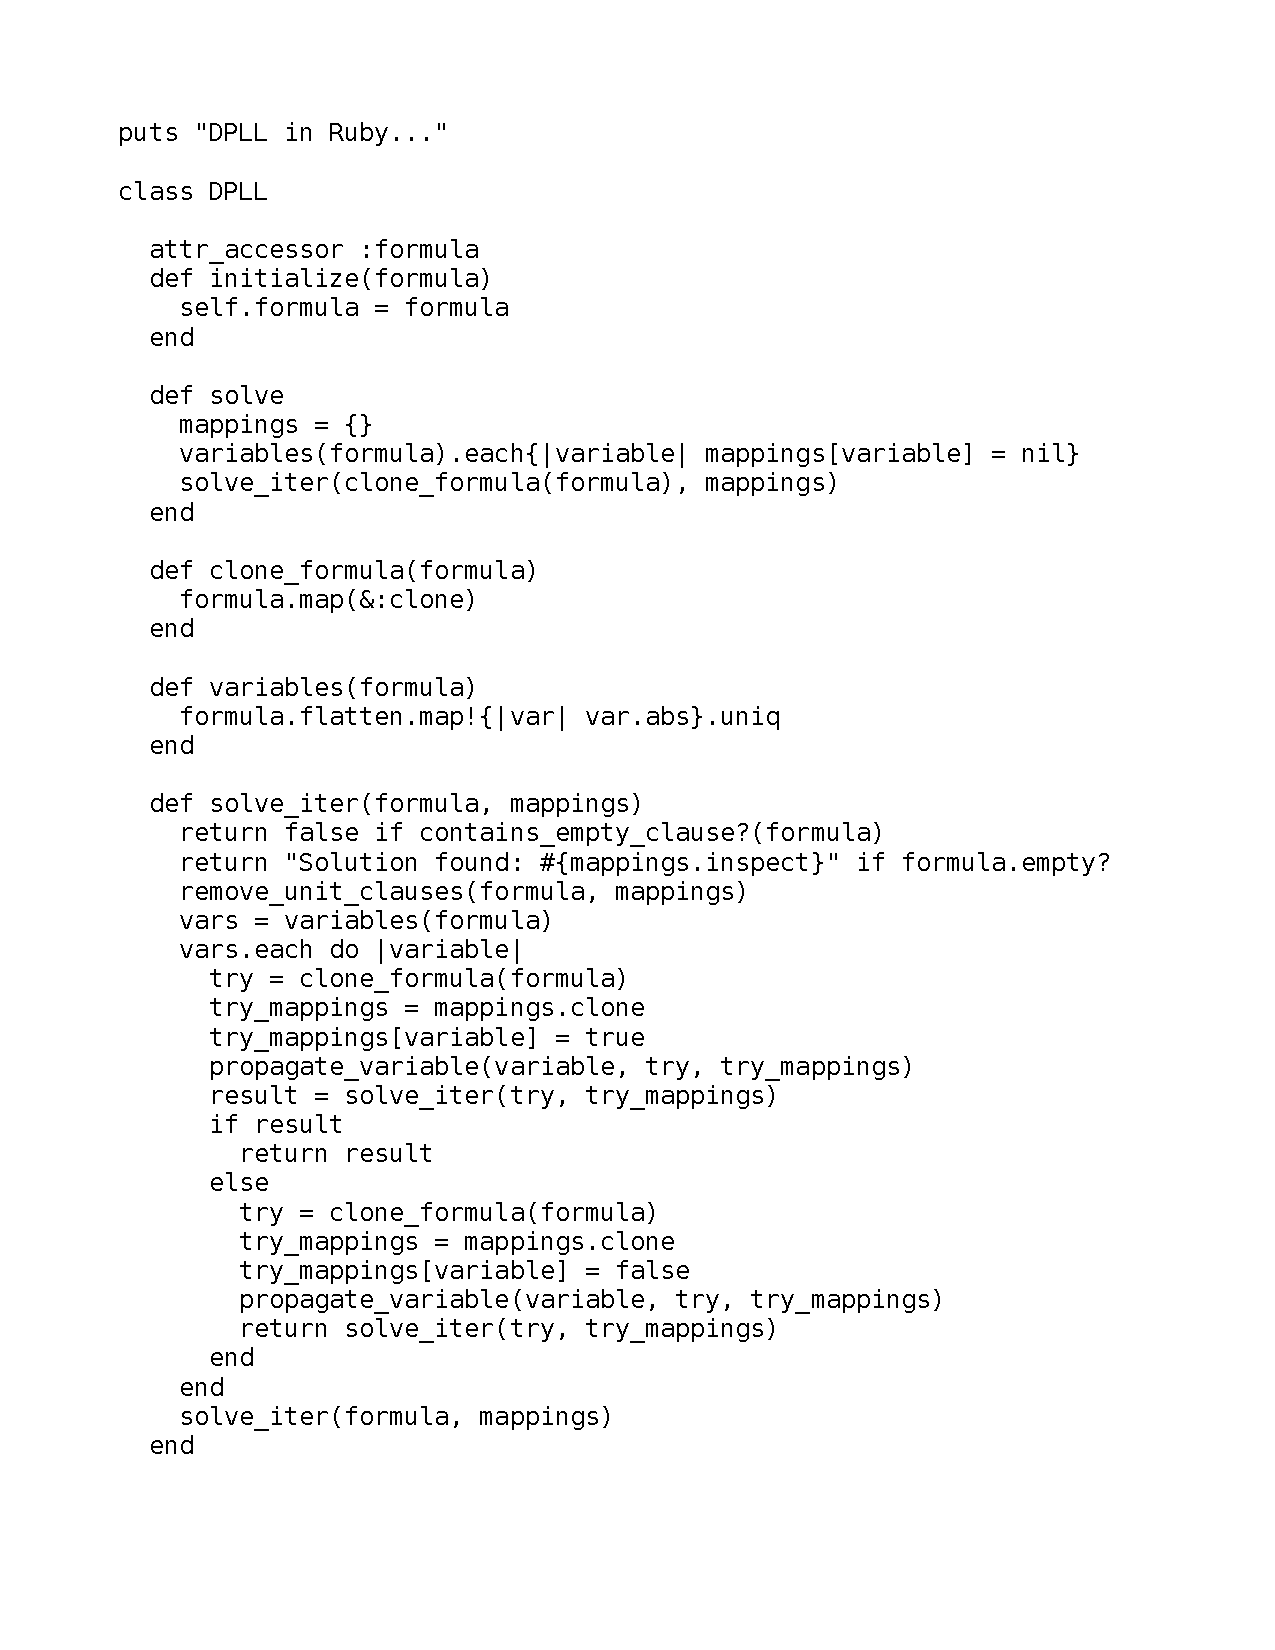
\includepdf[pages=-]{dpll.pdf}

\end{document}
